\documentclass{article}
\usepackage[table,xcdraw]{xcolor} % Dla tabel
\usepackage{siunitx} % Provides the \SI{}{} and \si{} command for typesetting SI units
\usepackage{graphicx} % Required for the inclusion of images
\usepackage{natbib} % Required to change bibliography style to APA
\usepackage{amsmath} % Required for some math elements 
\setlength\parindent{12pt} % Removes all indentation from paragraphs
%\usepackage{times} % Uncomment to use the Times New Roman font
\usepackage{amsmath}
\usepackage[export]{adjustbox}
\usepackage{tikz}
\usepackage{adjustbox}
\usepackage{caption}
\usepackage{pgfplots}
\usepackage[utf8]{inputenc} % Język polski
\usepackage{polski}
\usepackage[polish]{babel}

\usepackage[top=1in, bottom=1.25in, left=1.25in, right=1.25in]{geometry} % Marginesy
\usepackage{listings} % Kod programu
\usepackage{indentfirst} % Wcięcie przy pomocy \par
\usepackage{multicol} % Kilka kolumn dla itemize
\usepackage{color} % Kolorowanie tekstu
\usepackage{float}

\captionsetup{justification=centering}

%\renewcommand{\labelenumi}{\alph{enumi}.} % Zamienia litery w enumerate na a, b, c, ...
%----------------------------------------------------------------------------------------
%	DOCUMENT INFORMATION
%----------------------------------------------------------------------------------------
\title{Projektowanie Efektywnych Algorytmów \\ {\normalsize Implementacja i analiza efektywności metody Tabu Search dla problemu komiwojażera}}
\author{Sebastian Łągiewski 226173\\Łukasz Zatorski 226172 }

% Title page layout (fold)
\makeatletter
\renewcommand{\maketitle}{
	\begin{titlepage}
		\begin{center}
			\vspace*{3cm}
			\LARGE \@title \par
			\vspace{2cm}
			\textit{\small Autorzy:}\par
			\normalsize \@author\par \normalsize
			\vspace{3cm}
			Prowadzący : mgr inż. Radosław Idzikowski\\
			\vspace{3cm}
			Wydział Elektroniki\\ III rok \par
			\vspace{3cm}
			\small \@date
		\end{center}
	\end{titlepage}
}
\makeatother
\begin{document}
	\maketitle % Insert the title, author and date

%\begin{center}
%\begin{tabular}{l r}
%Data: & Semestr letni, 2017 \\ % Date the experiment was performed

%Prowadzący:  mgr inż. Radosław Idzikowski% Instructor/supervisor
%\end{tabular}
%\end{center}
\tableofcontents


% If you wish to include an abstract, uncomment the lines below
% \begin{abstract}
% Abstract text
% \end{abstract}

%----------------------------------------------------------------------------------------
%	SECTION 0
%----------------------------------------------------------------------------------------

%\newpage
%\section{Tytuł}} 
%\subsection{Tytuł}
%\par Tekst

%\begin{itemize}
%	\item\textit{Tekst} - Opis
%\end{itemize}

%\begin{enumerate}
%	\item Opis
%\end{enumerate}

%\begin{center}
%	\includegraphics[scale=0.6, center]{Screenshot_1.png}
%\end{center}

%\begin{lstlisting}[basicstyle=\small]
%	kod programu;
%\end{lstlisting}

%----------------------------------------------------------------------------------------
%	SECTION 1
%----------------------------------------------------------------------------------------
\newpage
\section{Opis algorytmu}
\par Tabu Search jest metaheurystyką do rozwiązywania problemów optymalizacyjnych, opartą na iteracyjnym przeszukiwaniu
przestrzeni rozwiązań, wykorzystującą ich sąsiedztwo, zapamiętującą niektóre ruchy oraz odległość czasową ich wystąpienia, w celu unikania minimów lokalnych i poszukiwania rozwiązań globalnie optymalnych w rozsądnym czasie.
\newline
\newline
Algorytm Tabu Search dla problemu komiwojażera polega na iteracyjnym przeszukiwaniu sąsiedztwa obecnie obecnie rozpatrywanego rozwiązania. Początkowe rozwiązanie generowane jest przy pomocy algorytmu zachłannego, dla losowo wybranego miasta początkowego. Następnie przez określoną liczbę iteracji, wykonywane są kolejne kroki algorytmu: 
	\begin{enumerate}
	\item Przeszukiwanie sąsiedztwa obecnie rozpatrywanego rozwiązania poprzez wielokrotną zamianę kolejności odwiedzenia dwóch losowo wybranych miast, a następnie wybranie tej zamiany, która nie należy do tabu oraz dla której droga jest najkrótsza.
	\item Dodanie do listy tabu zamiany prowadzącej do otrzymania najlepszego lokalnie rozwiązania.
	\item Porównanie najlepszego lokalnie rozwiązania dla danej iteracji z rozwiązaniem najlepszym globalnie. Jeżeli rozwiązanie lokalne jest lepsze od globalnego, nowym rozwiązaniem globalnym staje się obecne rozwiązanie lokalne.
\end{enumerate}

\textbf{Elementy charakterystyczne metody}
\begin{itemize}
	\item \textit{Lista ruchów będących tabu}.
	\item \textit{Zdarzenie krytyczne} - wywołanie określonej czynności, jeśli przez określony odstęp czasu rozwiązanie nie uległo poprawie.
	\item \textit{Strategia dywersyfikacji} - wygenerowanie nowego rozwiązania początkowego, na którym będą dokonywane zmiany. Jest wywoływana przez zdarzenie krytyczne.
	\item \textit{Strategia aspiracji} - ignorowanie ruchu znajdującego się na liście tabu, jeśli ma on szansę na przeniesienie poszukiwania na bardziej obiecujący obszar.
\end{itemize}
\newpage
\section{Plan eksperymentu}
\par
\begin{itemize}
\item Pomiar czasu został wykonany za pomocą klasy StopWatch(QueryPerformanceCounter).
\item Do reprezentacji odległości między miastami użyto macierzy sąsiedztwa.
\item Dla każdego z typów pomiaru algorytm wykonywany był 30 razy, wyniki uśredniono.
\end{itemize}

\textbf{Metoda Tabu Search}
\renewcommand\labelitemii{$\circ$}
\begin{itemize}
	\item Do przechowywania listy tabu użyto macierzy \textit{N}x\textit{N}, gdzie \textit{N} - liczba miast rozpatrywanego przypadku. Współrzędne \textit{[i, j]} oznaczają zamianę  kolejności elementu \textit{i} z elementem \textit{j}.
	\item Zdarzenie krytyczne polega na wywołaniu dywersyfikacji, jeśli przez \textit{x} ostatnich iteracji głównej pętli nie nastąpiła poprawa najlepszego rozwiązania.
	\item Dywersyfikacja polega na obraniu nowego rozwiązania początkowego, na którym będą dokonywane zmiany. Rozwiązanie to jest generowane przy użyciu algorytmu zachłannego, dla losowo wybranego miasta początkowego.
	\item Kryterium aspiracji anuluje zakaz ruchu, jeśli spełniony jest warunek dla danego rozwiązania lokalnego: \textit{x} * \textit{1.05} $<$  \textit{y}, gdzie \textit{x} - waga obecnie rozpatrywanego rozwiązania lokalnego, \newline \textit{y} - waga obecnie najlepszego rozwiązania lokalnego.
\end{itemize}
\newpage

\section{Wyniki}

\subsection{Wpływ strategii dywersyfikacji na działanie algorytmu}
\begin{figure}[H]
\begin{adjustbox}{addcode={\begin{minipage}{\width}}{\caption{%
					Wpływ strategii dywersyfikacji na działanie algorytmu.
		}\end{minipage}},rotate=90,center}
	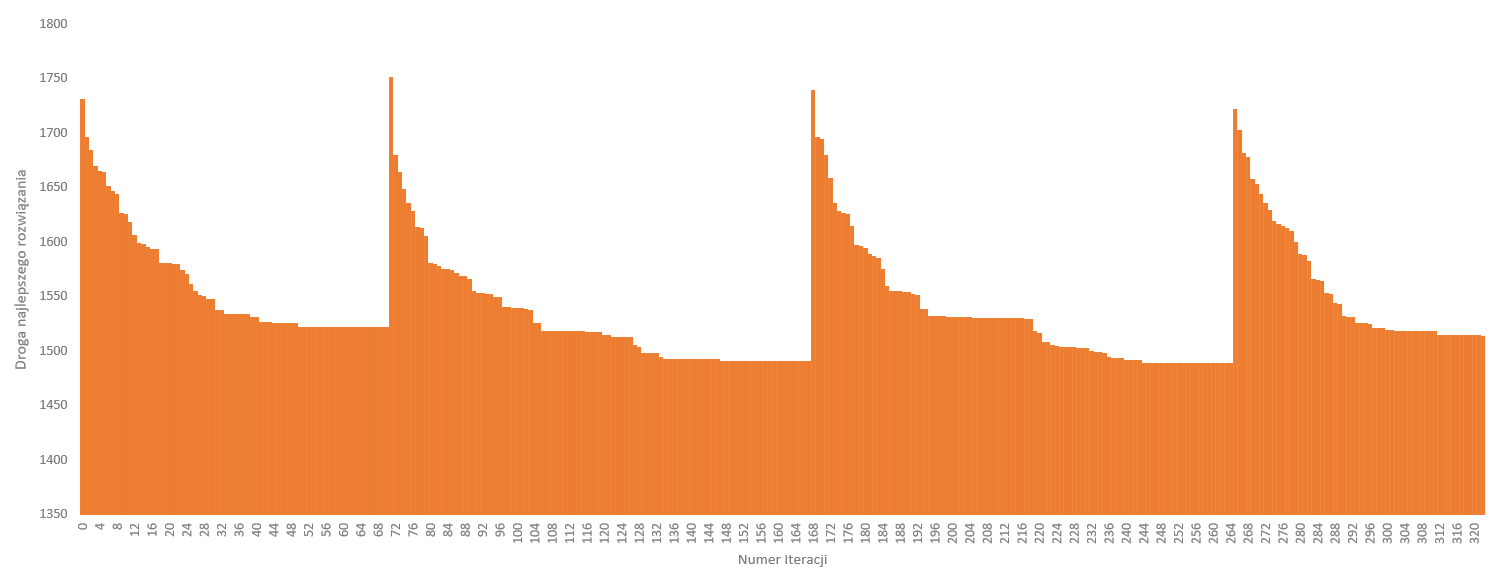
\includegraphics[scale=.5]{NowyToBest.png}%
\end{adjustbox}
\end{figure}
\newpage
\par W celu zilustrowania wpływu strategii dywersyfikacji na działanie napisanego algorytmu, przyjęto, iż po zdarzeniu krytycznym nowym najlepszym rozwiązaniem zostanie nowo wygenerowane rozwiązanie startowe(za pomocą algorytmu zachłannego).

\subsection{Zależność jakości rozwiązania od czasu(ilości iteracji) znajdowania się wybranych ruchów na liście tabu}
\begin{table}[H]
	%\vspace{cm}
	\centering
	%\label{my-label}
	
	\begin{tabular}{|c|c|}
		\hline
		\multicolumn{1}{|c|}{\textbf{Timestamp}} & \textbf{Błąd względny wyniku (\%)}  \\ \hline
		{10}                                	& 19,88               \\ \hline
		{60}                                & 20,59               \\ \hline
		{110}                                & 21,15                \\ \hline
		{160}                                & 20,71                 \\ \hline
		{210}                                & 22,07                 \\ \hline
	\end{tabular}
	\caption{Zależność jakości rozwiązania od czasu(ilości iteracji) znajdowania się wybranych ruchów na liście tabu, dla instancji rbg323}
\end{table}	

\begin{figure}[h]
	\centering
	\vspace{0.75cm}
	\hspace*{-0.8cm}
	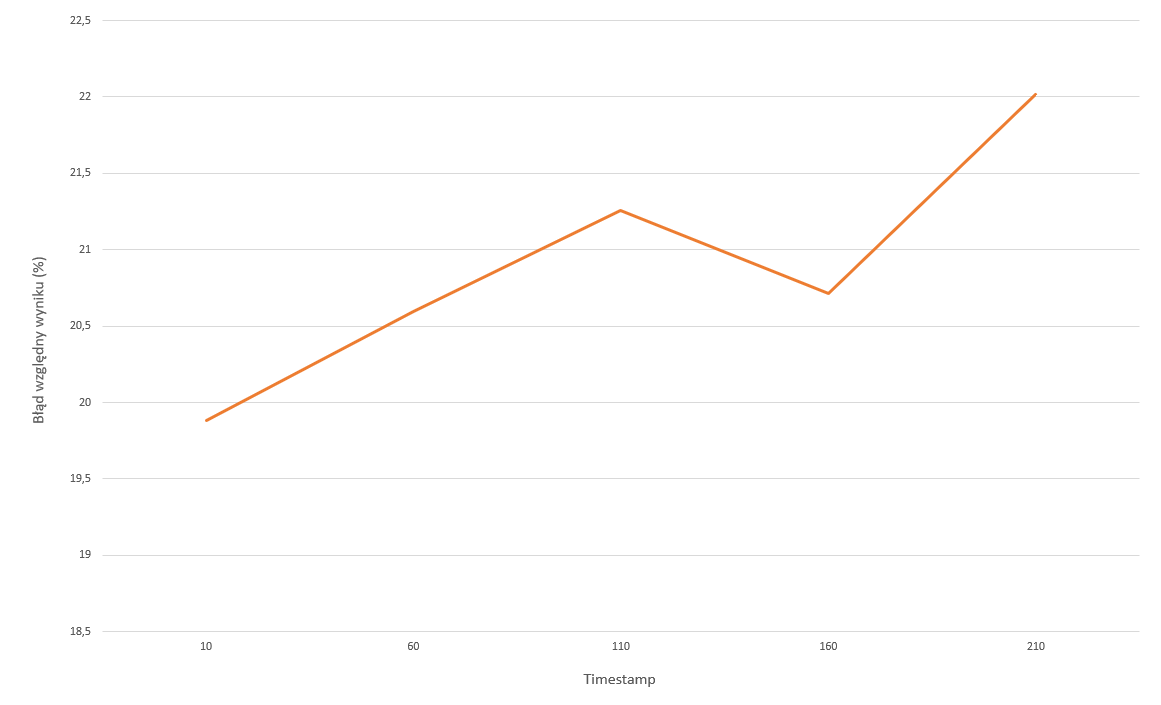
\includegraphics[scale=0.55]{wplywTimestamp.png}
	\caption{Wpływ jakości rozwiązania od czasu(ilości iteracji) obecności wybranych ruchów na liście tabu, dla instancji rbg323.}
	%\label{fig:obrazek k}
\end{figure}

\subsection{Zależność jakości rozwiązania od długości wykonywania się algorytmu}
\subsubsection{rat783}
\begin{figure}[H]
	\begin{adjustbox}{addcode={\begin{minipage}{\width}}{\caption{%
						Zależność błędu względnego rozwiązania od długości wykonywania algorytmu(ilości iteracji). Czas ograniczono do 2 minut.
			}\end{minipage}},rotate=90,center}
		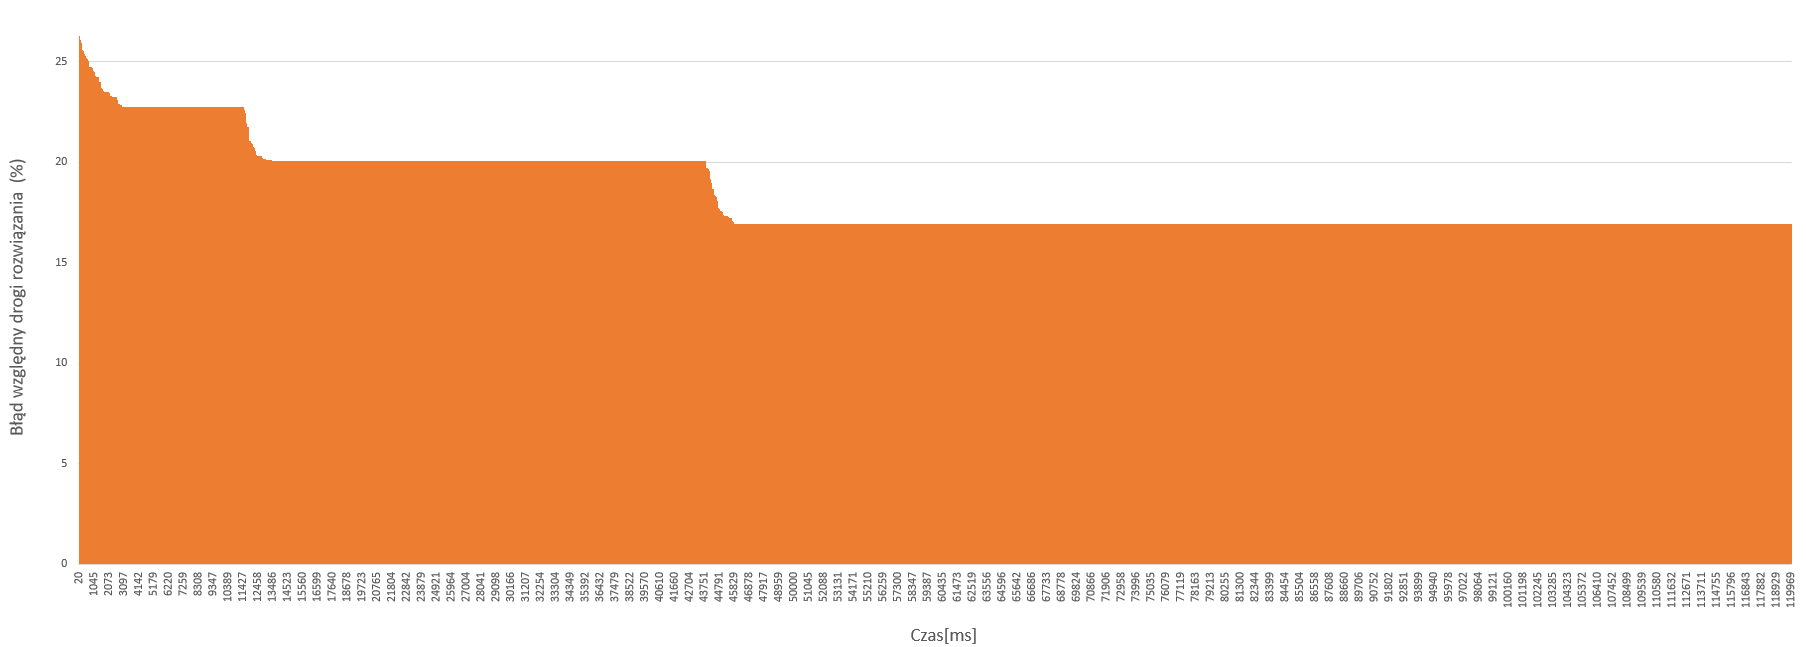
\includegraphics[scale=.43]{rat783_odCzasu.png}%
	\end{adjustbox}
\end{figure}

\newpage
\subsubsection{pr1002}
\begin{figure}[H]
	\begin{adjustbox}{addcode={\begin{minipage}{\width}}{\caption{%
						Zależność błędu względnego rozwiązania od długości wykonywania algorytmu(ilości iteracji). Czas ograniczono do 2 minut.
			}\end{minipage}},rotate=90,center}
		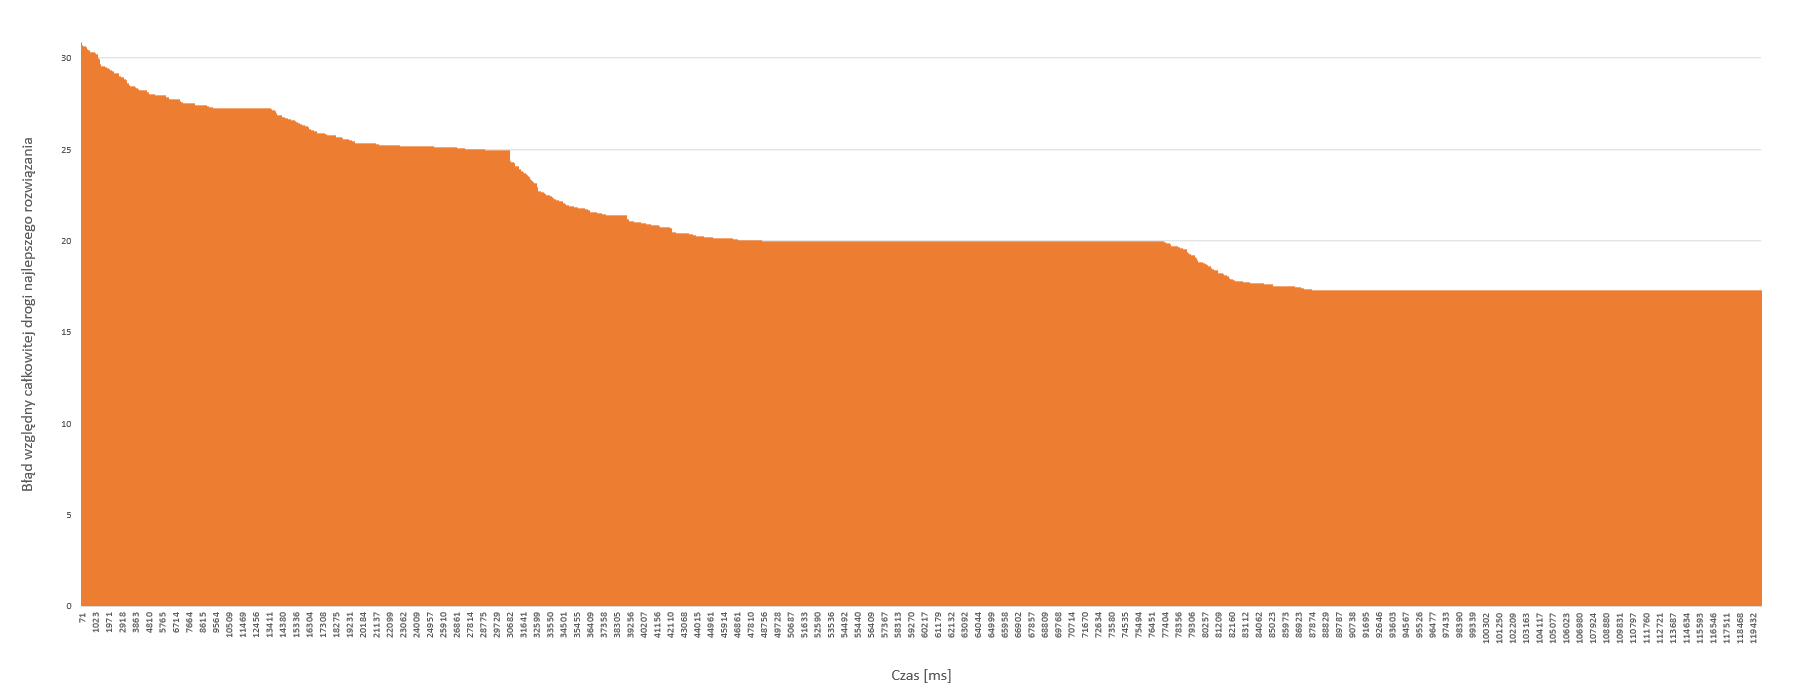
\includegraphics[scale=0.45]{pr1002_odCzasu.png}%
	\end{adjustbox}
\end{figure}

\newpage
\subsubsection{d2103}
\begin{figure}[H]
	\begin{adjustbox}{addcode={\begin{minipage}{\width}}{\caption{%
						Zależność błędu względnego rozwiązania od długości wykonywania algorytmu(ilości iteracji). Czas ograniczono do 3 minut.
			}\end{minipage}},rotate=90,center}
		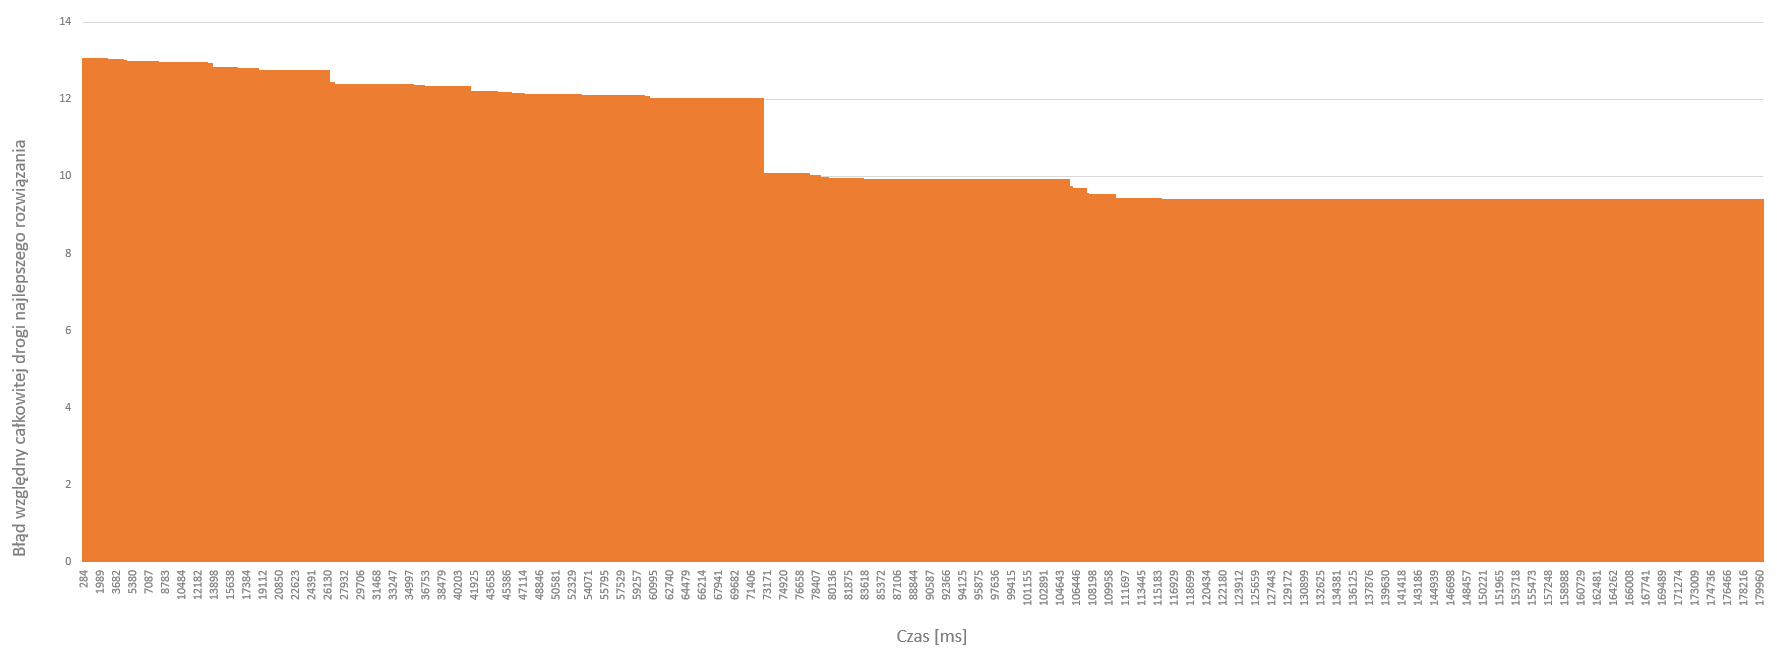
\includegraphics[scale=.45]{d2103_odCzasu.png}%
	\end{adjustbox}
\end{figure}




%\begin{figure}[H]
%	\centering
%	\includegraphics[scale=0.5, center]{Screenshot_1.png}
%	\caption{Zależność czasu wykonania się algorytmu od liczby miast}
%\end{figure}
	%


\newpage	
	
\section{Podsumowanie}
\par	
	
	



%----------------------------------------------------------------------------------------
%	SECTION 3
%----------------------------------------------------------------------------------------

%----------------------------------------------------------------------------------------
%	SECTION 4
%----------------------------------------------------------------------------------------

%----------------------------------------------------------------------------------------
%	BIBLIOGRAPHY
%----------------------------------------------------------------------------------------
%\newpage
%\bibliohystyle{apalike}
%\begin{thebibliography}{9}
%
%\bibitem{wikipediacluster} 
%Wikipedia: Computer cluster,
%\\\texttt{https://en.wikipedia.org/wiki/Computer\_cluster}
%	
%\bibitem{wikipediasieve} 
%Wikipedia: Sieve of Erastosthenes,
%\\\texttt{https://en.wikipedia.org/wiki/Sieve\_of\_Eratosthenes}
%
%\end{thebibliography}

%----------------------------------------------------------------------------------------
\end{document}
